% Problema:
\begin{frame}{El problema.} %%Otra forma (más corta) de poner el título a la diapositiva
  \framesubtitle{¿Cuántas lámparas son necesarias para iluminar?} %%Subtítulo de la diapositiva (opcional)
  \begin{teorema}
    $\lfloor \frac{n}{4} \rfloor$ lámparas son siempre son siempre suficientes y a veces necesarias
    para iluminar cualquier polígono ortogonal con $n$ vértices.
  \end{teorema}
\end{frame}

% Demostración:
\begin{frame}{El problema.} %%Otra forma (más corta) de poner el título a la diapositiva
  \framesubtitle{¿Cuántas lámparas son necesarias para iluminar?} %%Subtítulo de la diapositiva (opcional)
  \textbf{Demostración:}
    Sea $P$ de al menos $8$ vértices. Sean $S_1$ y $S_2$ conjuntos tales que contengan los vértices superiores derechos; inferiores izquierdos
    y los superiores izquierdos; inferiores derechos, respectivamente. $S_1$ o $S_2$ contiene a lo más $\lfloor \frac{n}{4} \rfloor$ vértices
    concavos. Supongamos que es $S_1$ quién contiene a lo más $\lfloor \frac{n}{4} \rfloor$ vértices concavos.
    Si esos vértices iluminan a $P$, entonces terminamos.\newline
    
    Supongamos que los vértices concavos de $S_1$ no iluminan $P$. Entonces, mostremos que existe un corte vértical u horizontal impar.
    Sean, $p \in P$ tal que no es iluminado por algún $s \in S_1$; c un segmento horizontal (vértical) más largo que contiene a $p$;
    $e, f$ aristas de $P$ que contienen los extremos de $c$. $R$ es el rectángulo más grande contenido en $P$ con lados paralelos a
    los ejes coordenados que contenga a $c$.\newline
\end{frame}

\begin{frame}{El problema.} %%Otra forma (más corta) de poner el título a la diapositiva
  \framesubtitle{¿Cuántas lámparas son necesarias para iluminar?} %%Subtítulo de la diapositiva (opcional)
  \textbf{Obs.} Sean $q, q'$ los vértices \textit{superior derecho} e \textit{inferior izquierdo} respectivamente.
  Si $q, q' \in V_P \rightarrow P = R$.

  \begin{figure}
    \centering
    \begin{subfigure}[b]{0.59\paperwidth}
      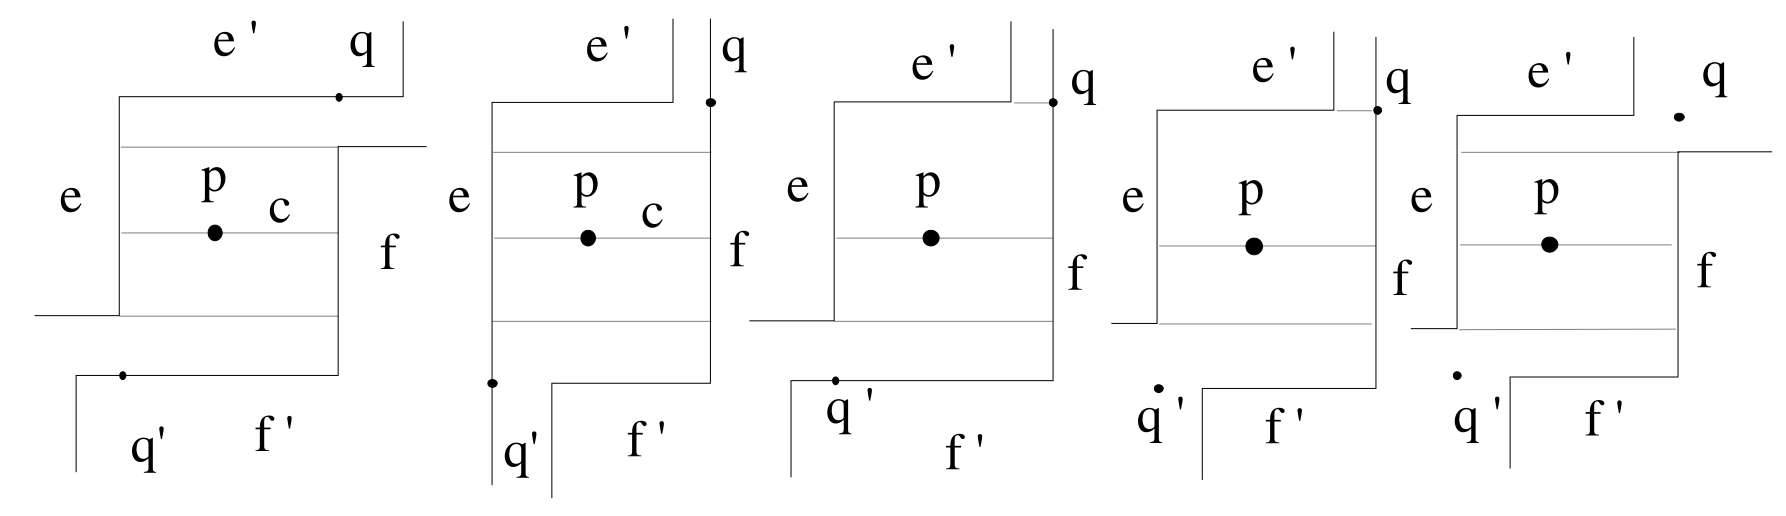
\includegraphics[width=.6 \paperwidth]{./images/CasosOrtogonales.png}
    \end{subfigure}
    \begin{subfigure}[b]{0.1\paperwidth}
      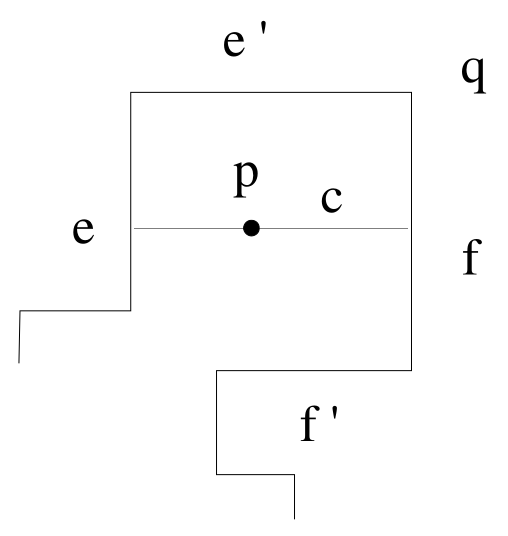
\includegraphics[width=.16 \paperwidth]{./images/CasoOrtogonal.png}
    \end{subfigure}
    \caption*{Casos generados por $q$ y $q'$.}
  \end{figure}
\end{frame}

\begin{frame}{El problema.} %%Otra forma (más corta) de poner el título a la diapositiva
  \framesubtitle{¿Cuántas lámparas son necesarias para iluminar?} %%Subtítulo de la diapositiva (opcional)
  Analicemos $2$ posibles casos:
  \begin{itemize}
  \item $q$ y $q'$ no son vértices de $P$.
  \item Exactamente uno de ellos, digamos que $q$, es vértice de $P$.
  \end{itemize}
  \begin{figure}
    \centering
    \begin{subfigure}[b]{0.59\paperwidth}
      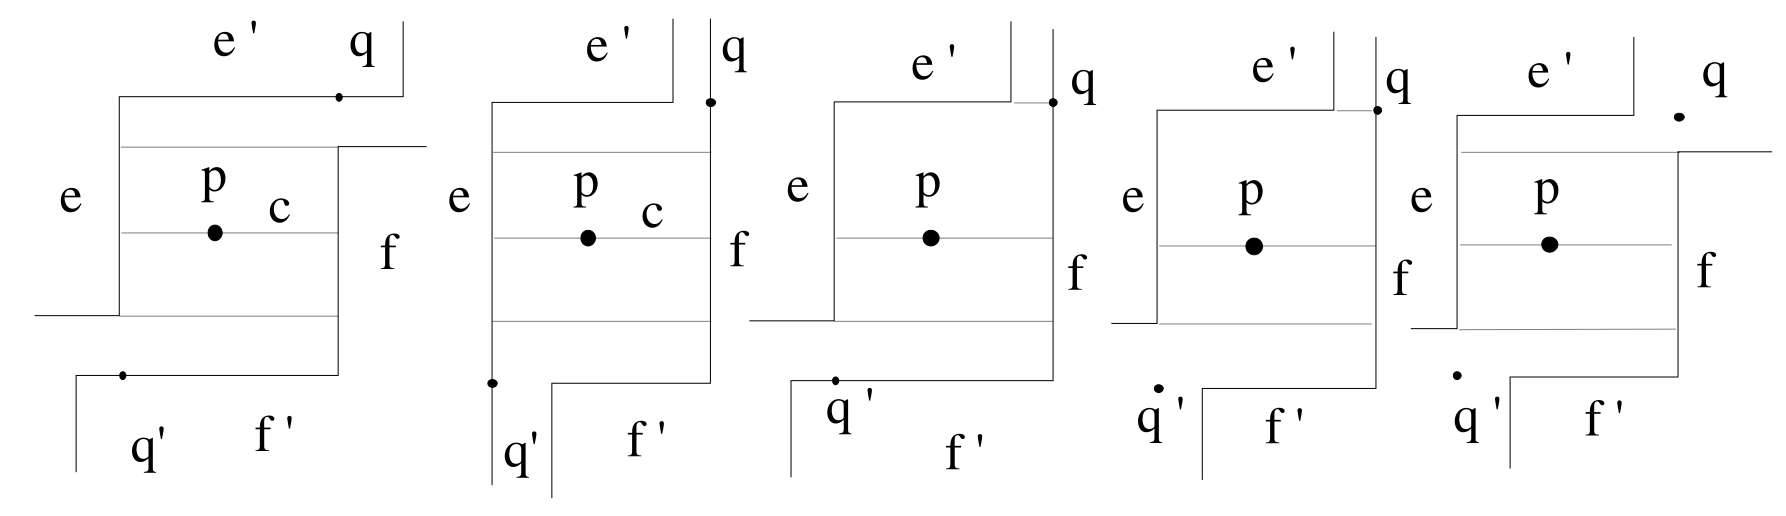
\includegraphics[width=.6 \paperwidth]{./images/CasosOrtogonales.png}
    \end{subfigure}
    \begin{subfigure}[b]{0.1\paperwidth}
      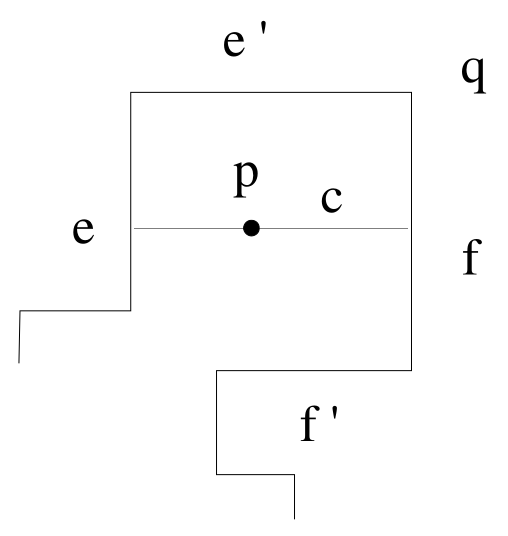
\includegraphics[width=.16 \paperwidth]{./images/CasoOrtogonal.png}
    \end{subfigure}
    \caption*{Casos generados por $q$ y $q'$.}
  \end{figure}
\end{frame}

\begin{frame}{El problema.} %%Otra forma (más corta) de poner el título a la diapositiva
  \framesubtitle{¿Cuántas lámparas son necesarias para iluminar?} %%Subtítulo de la diapositiva (opcional)
  Para el caso (1) es fácil ver que podemos generar dos cortes vérticales (horizontales) en $P$ que generen $R$
  o un rectángulo contenido en el y que contiene a $c$. Es sencillo observar que al menos un corte es impar.
  \begin{figure}
    \centering
    \begin{subfigure}[b]{0.25\paperwidth}
      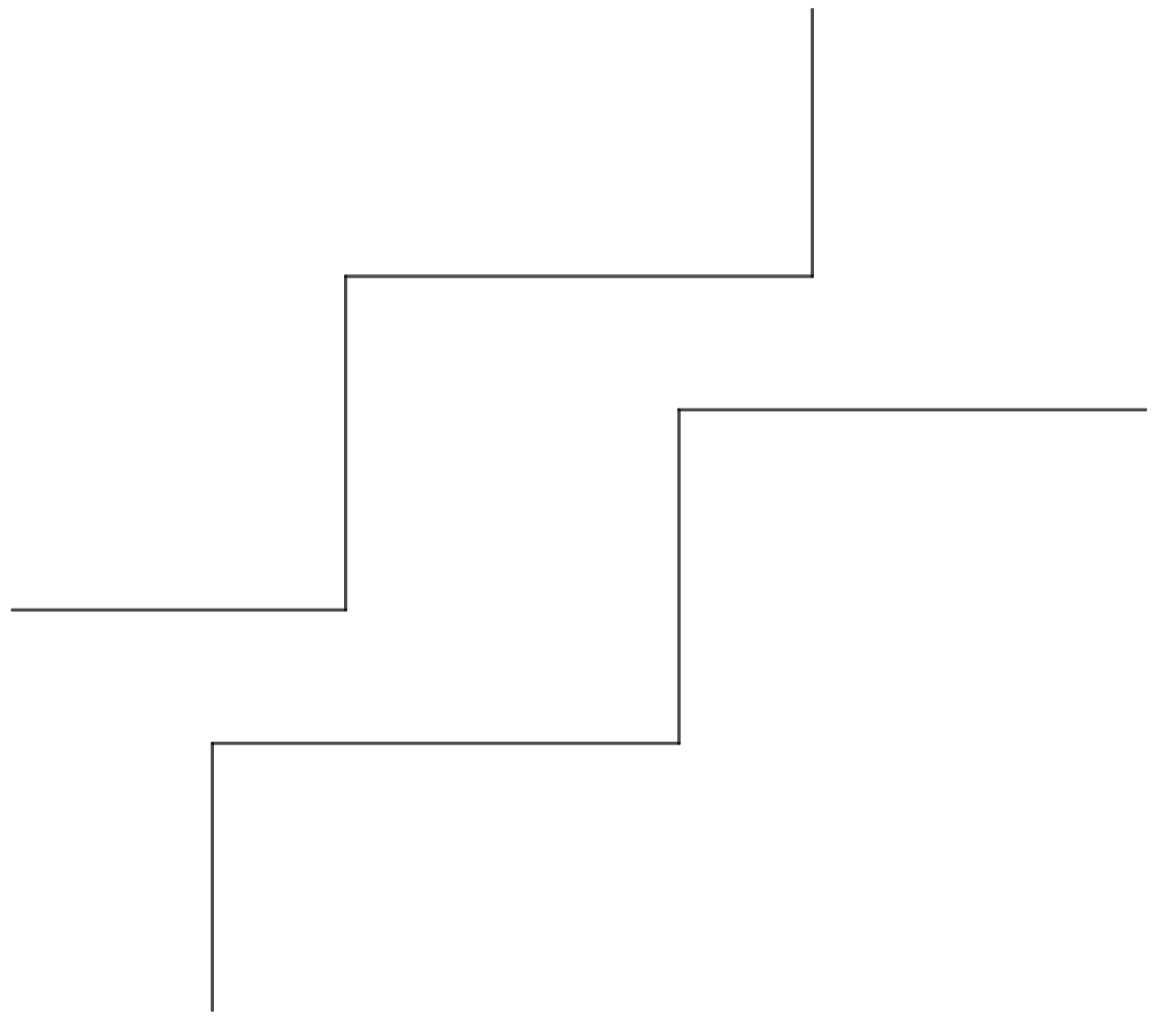
\includegraphics[width=.3 \paperwidth]{./images/Ejemplar.png}
    \end{subfigure}
    \begin{subfigure}[b]{0.25\paperwidth}
      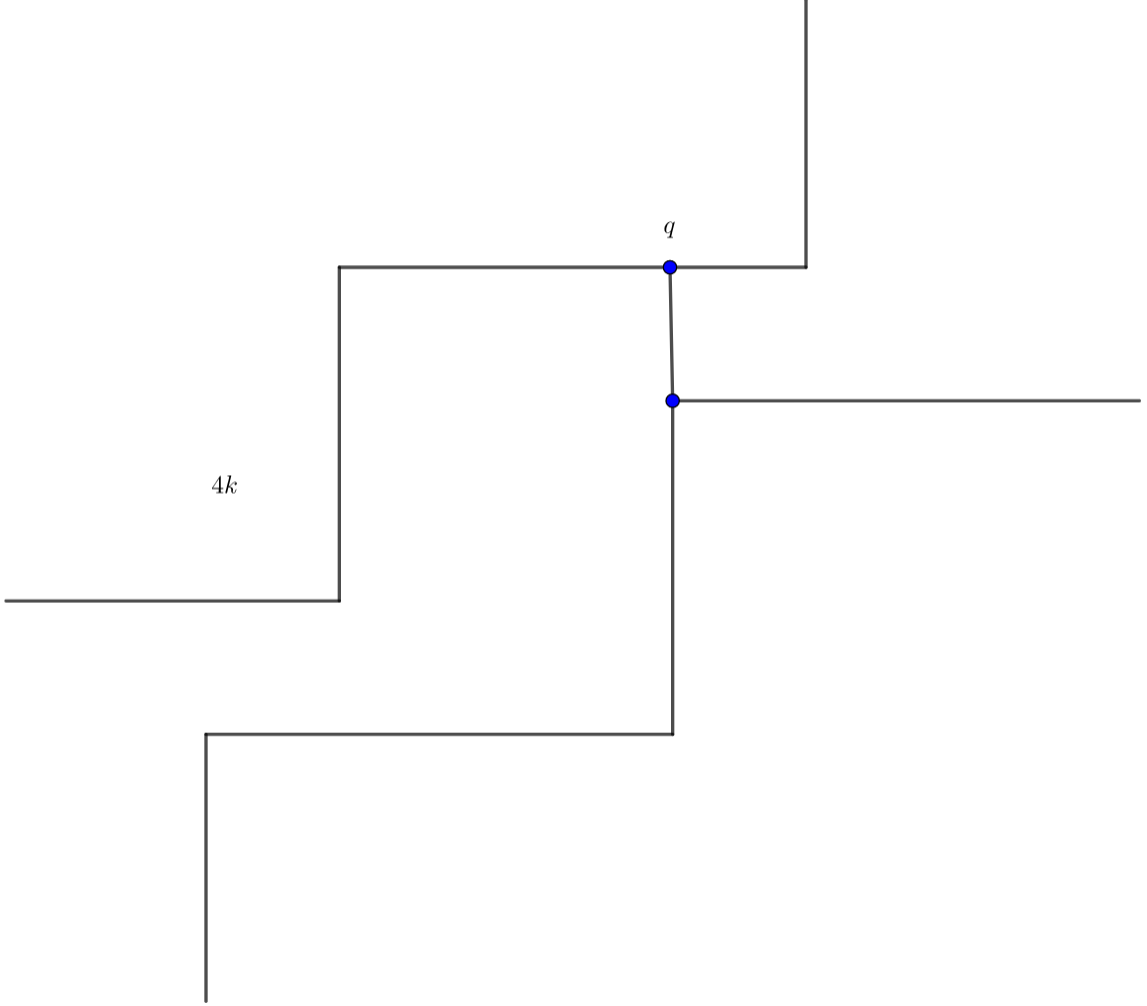
\includegraphics[width=.3 \paperwidth]{./images/EjemplarC1(4k).png}
    \end{subfigure}
    \begin{subfigure}[b]{0.25\paperwidth}
      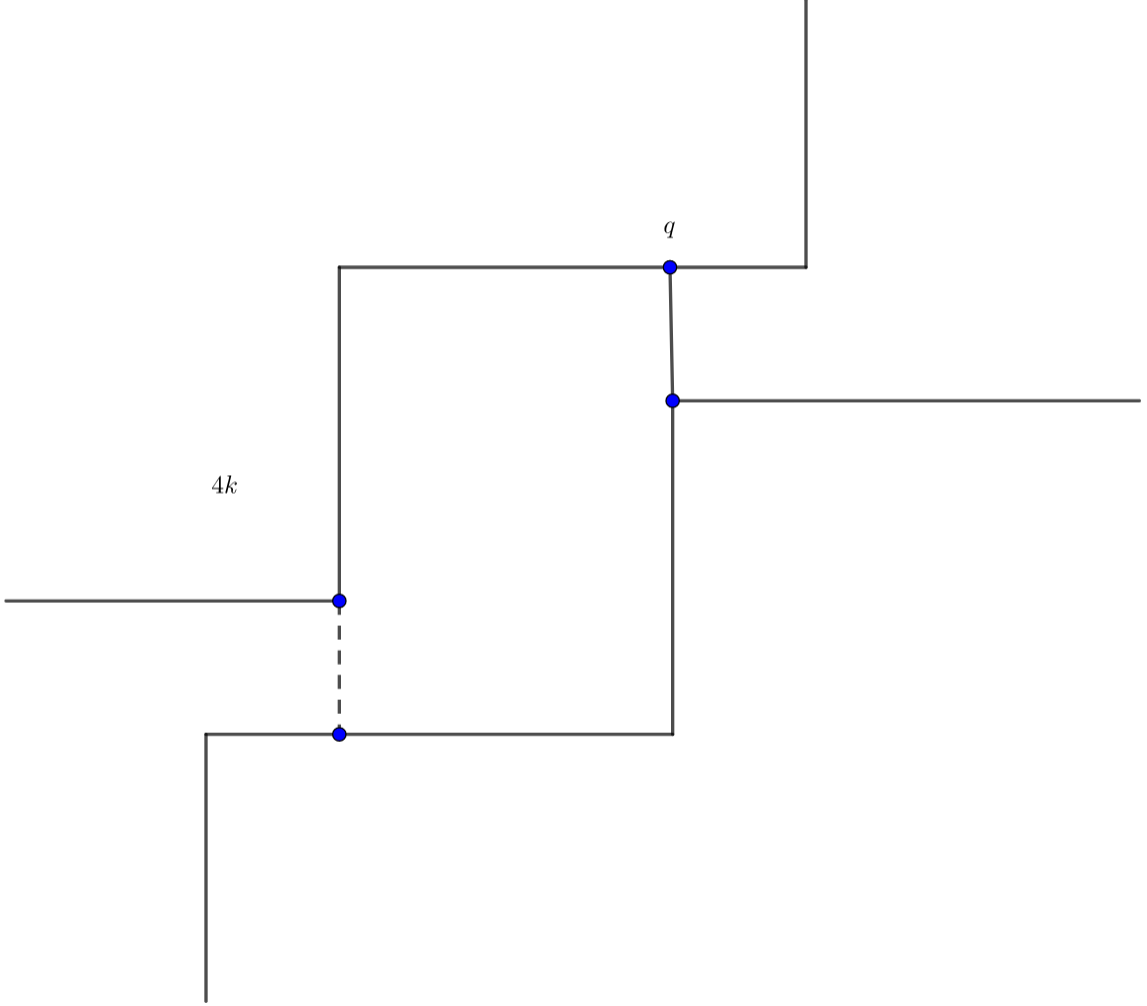
\includegraphics[width=.3 \paperwidth]{./images/EjemplarC1.png}
    \end{subfigure}
    \caption*{Suponemos que el primer corte genera a un corte de tamaño $4k$.}
  \end{figure}
  De lo anterior tenemos $4k - 3 + 1 = 4k - 2 = 4k' + 2$.\newline
  
\end{frame}

\begin{frame}{El problema.} %%Otra forma (más corta) de poner el título a la diapositiva
  \framesubtitle{¿Cuántas lámparas son necesarias para iluminar?} %%Subtítulo de la diapositiva (opcional)
  Otro posibles caso es
  \begin{figure}
    \centering
    \begin{subfigure}[b]{0.25\paperwidth}
      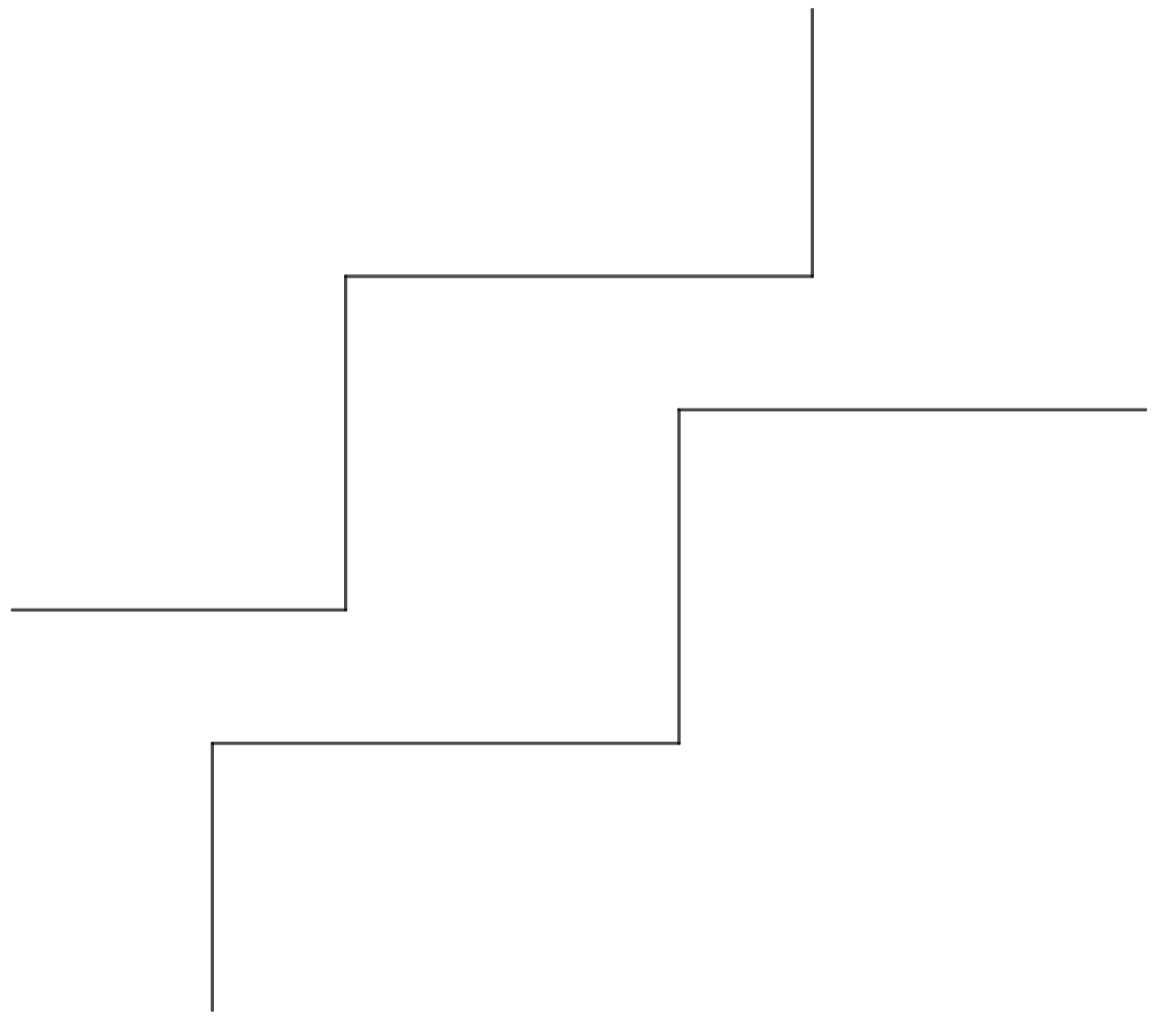
\includegraphics[width=.3 \paperwidth]{./images/Ejemplar.png}
    \end{subfigure}
    \begin{subfigure}[b]{0.25\paperwidth}
      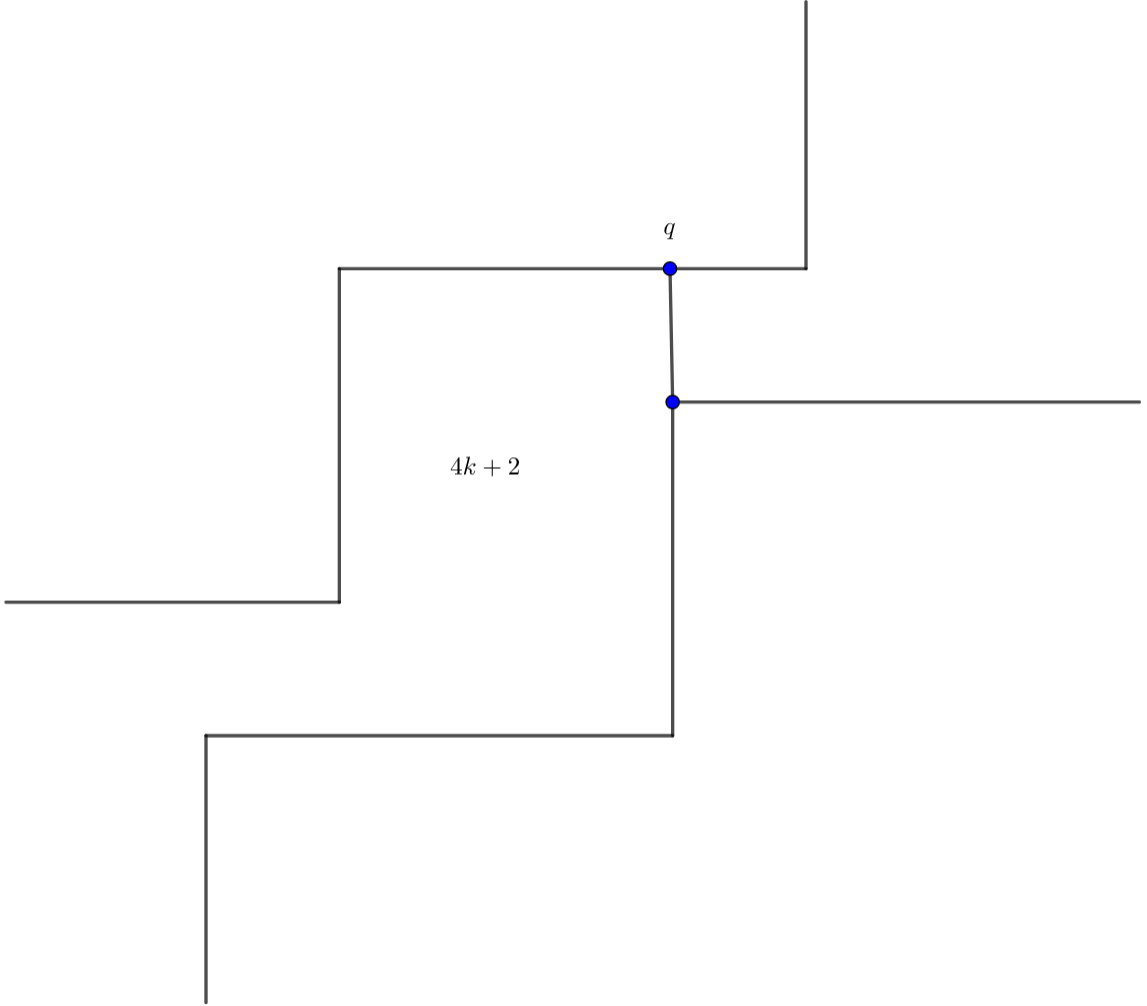
\includegraphics[width=.3 \paperwidth]{./images/EjemplarC2.png}
    \end{subfigure}
    \begin{subfigure}[b]{0.25\paperwidth}
      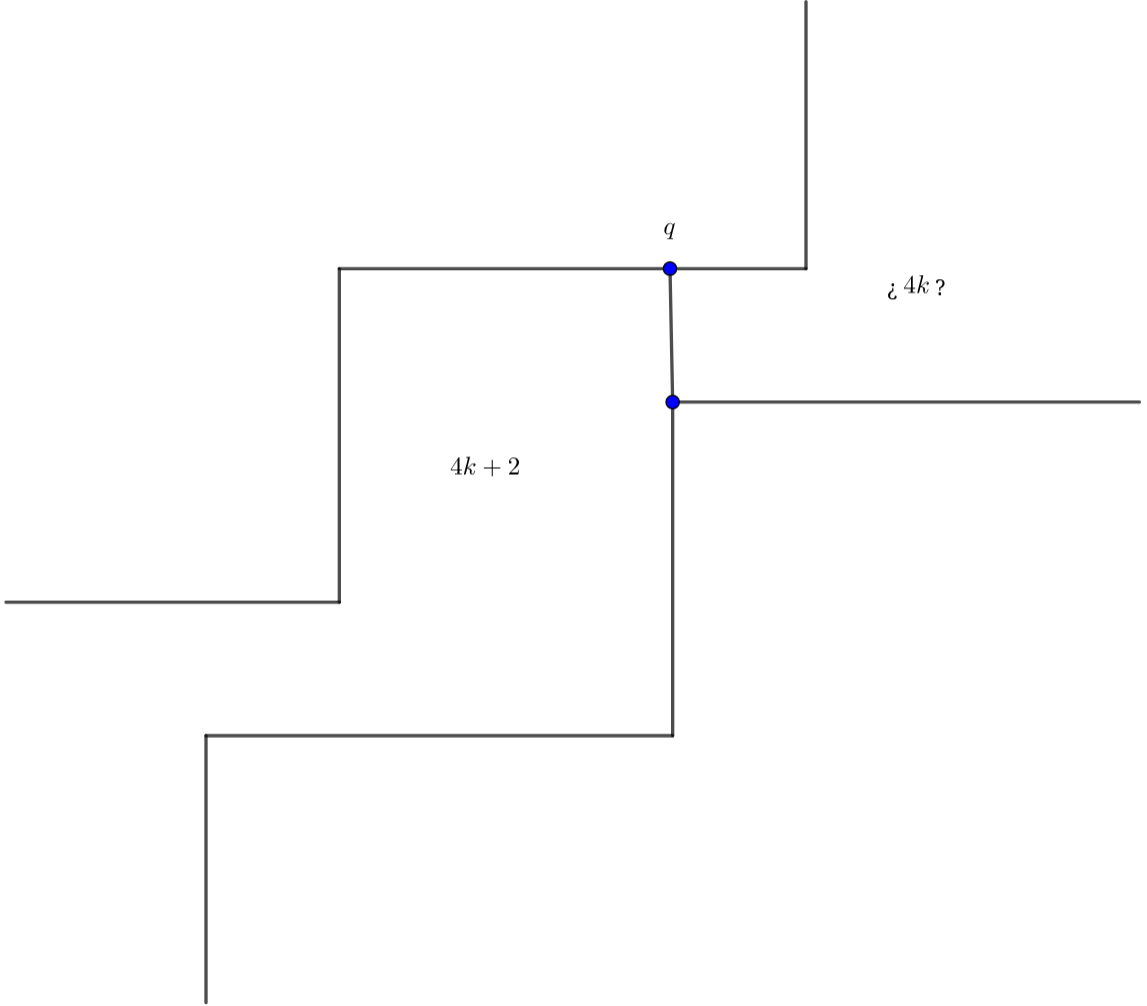
\includegraphics[width=.3 \paperwidth]{./images/EjemplarC2(4k + 2).png}
    \end{subfigure}
    \caption*{Suponemos que ambos cortes generan polígonos de tamaño $4k$.}
  \end{figure}
  De lo anterior tenemos
  \[(4k + 2 - 1) + (4k' - 1) - 1 = 4(k + k') - 1 = 4k'' - 1 \:\: !!!\]
  \newline
  
\end{frame}

\begin{frame}{El problema.} %%Otra forma (más corta) de poner el título a la diapositiva
  \framesubtitle{¿Cuántas lámparas son necesarias para iluminar?} %%Subtítulo de la diapositiva (opcional)
  Para el caso (2) basta extender $e$ y $f'$ hasta que se intersecten y obtenemos un polígno de $n - 4$ vértices
  tal que por inducción se puede iluminar con $\lfloor \frac{n - 4}{4} \rfloor$ lámparas. Por tanto terminamos. \hfill $\square$
  \begin{figure}
    \centering
    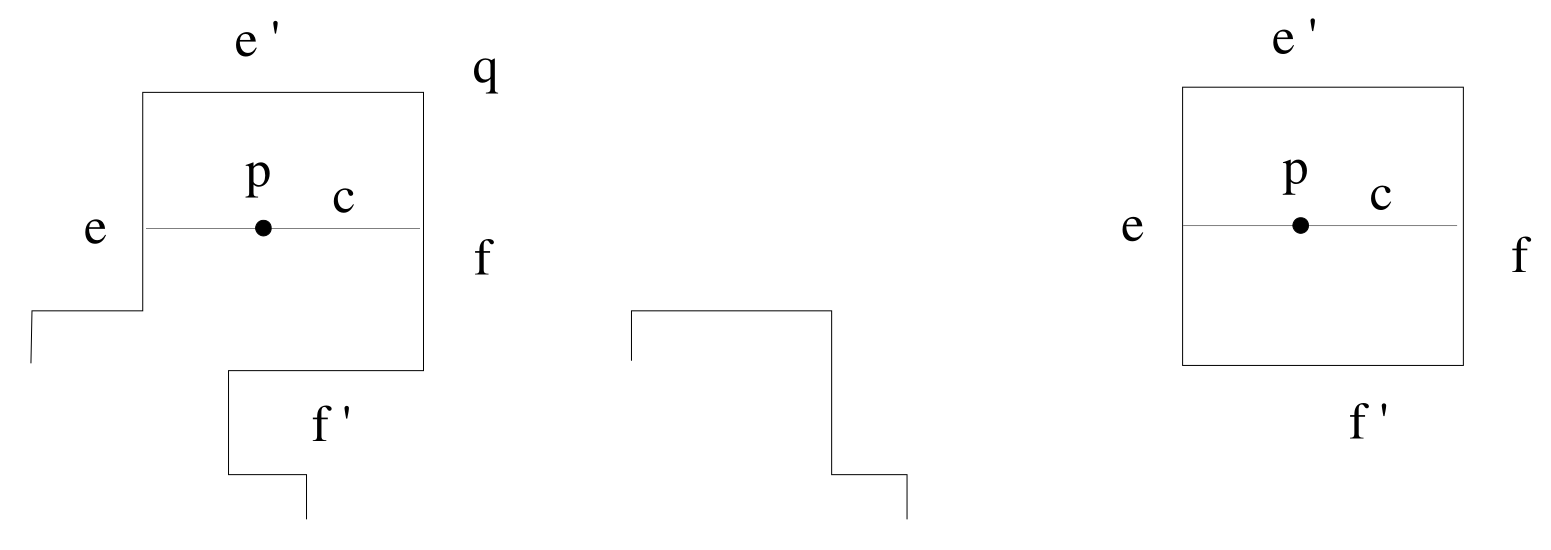
\includegraphics[width=.8 \paperwidth]{./images/Caso2.png}
    \caption*{Bosquejo del punto 2.}
  \end{figure}
\end{frame}
